\section{Method \& Theory}\label{method_theory}
\subsection{Stellar population in GC}\label{cmd_theory}
The typical stellar components of a \ac{GC} can be seen in a \ac{CMD}. In this \ac{CMD} the visual magnitude is plotted against the B-V color. It's color coded by the mass of the star. 
\begin{figure}[htbp]
\centering
	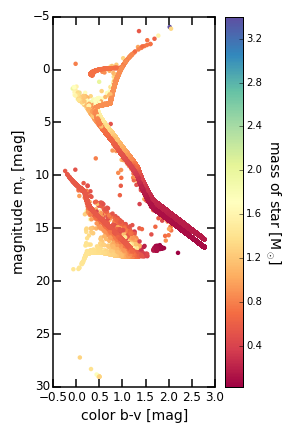
\includegraphics[width=0.5\textwidth]{Plots/color_magnitude_diagram.png}
	\caption{Color magnitude diagram of SIM 1.}
	\label{fig:cmd}
\end{figure}
A star's position can be interpreted as its evolution stage. Most of the stars are set in the main sequence. They fusion hydrogen in their cores. There are two main sequence lines one upon the other. These occur due to binary systems whose flux is given by the sum of the single fluxes of the single components, and therefore appear redder and more luminous. These binary systems represent about 5\% of the stars in the \ac{GC}. The position of the main sequence turn-off depends on the age of the system and therefore can be used as an indicator to determine the cluster's age. \color{red} explain isochrones \color{black} Bluewards of this turn off point following the trend of main sequence stars, there are so called "blue stragglers" which are remnants of stellar collisions or interacting binaries (B\&T p.628). Continuing from the turn off point there is the red giant branch consisting of stars still fusing hydrogen but only in a shell surrounding a degenerate helium core. They are inflated with a radius much higher than the main sequence stars but have a much lower temperature. These are the brightest stars of a \ac{GC}. On the upper part of the red giant branch lies the horizontal branch. Its stars burn helium in their core and hydrogen in a surrounding shell. In the lower left corner white dwarfs are located. They are stellar remnants which have burnt all of their resources. In a typical \ac{GC} dark stellar remnants like stellar black holes and neutron stars are present but not visualised in the \ac{CMD}. \color{red} nochmal über \ac{CMD} durchlesen\color{black} 
\subsection{Kinematic profiles of globular clusters}\label{kin_prof_theory}
\color{red} velocities are gauss distributed assumption \color{black}
Our investigations of \acp{GC} in phase space consists in analysing the spatial distribution of stars (density profiles) and the kinematic profiles(such as velocity dispersion and anisotropy profiles). First we test the sphericity of the \ac{GC}. Sphericity implies the usage of analytical methods that are very straight forward, especially for determing the potential of the globular cluster and then the actions in action space.\par \color{red} density profile \color{black} \par The velocity dispersion is the standard deviation of the mean velocity 
\begin{equation}
\sigma_i=\sqrt{\left\langle(v_i-\langle v_i\rangle)^2\right\rangle}=\sqrt{\left\langle v_i^2-\langle v_i\rangle^2\right\rangle} \qquad\qquad i=r,\theta,\phi.
\end{equation} For a spherical system it is best to calculate them in spherical coordinates \(r,\theta,\phi\) respectively \(v_r,v_{\theta},v_{\phi}\). If the \ac{GC} contains an \ac{IMBH} the velocity dispersion towards the centre is expected to increase. 
\par \color{red} what exactly describes anisotropy? \color{black} To quantify the anisotropy of the system we use the anisotropy parameter \(\beta\) 
\begin{equation}
\beta(r)\equiv1-\frac{\sigma_\theta ^2(r)+\sigma_\phi ^2(r)}{2\sigma_r ^2(r)}.
\end{equation} If \(\beta\) is positive the anisotropy is radial, if it is negative the anisotropy is tangential and if \(\beta\approx0\) then the system is isotropic.
\subsection{Density \& potential}\label{dens_pot_theory}
\begin{figure}[htbp]
\centering
	\begin{subfigure}{0.475\textwidth}
	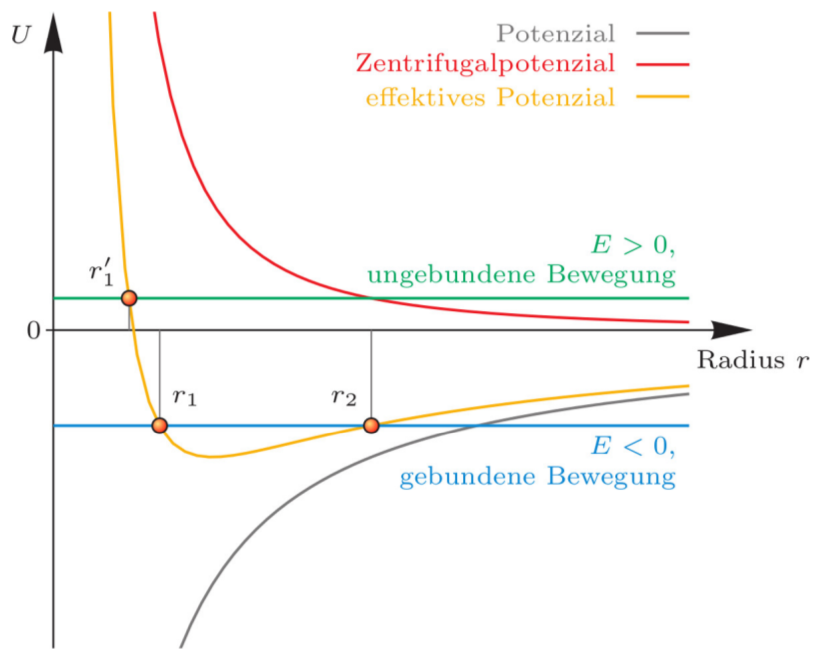
\includegraphics[width=\textwidth]{Plots/eff_potential_bartelmann.png}
	\caption{General potential of a central field. The black line is the potential which is the difference between the effective potential (yellow line) and the centrifugal potential (red line). If the effective potential is positive the object is unbound while having a negative potential the object moves on a bound orbit. The points where the effective potential equals the total energy are the peri- and apocentre (r\(_1\) and r\(_2\)) of the orbit. The point with the lowest effective potential is the guiding star radius. This is the distance a star with given angular momentum would have on a circular orbit. [Bartelmann Skript Theo 1]}
	\label{fig:eff_potential_bartelmann}
	\end{subfigure}
	\hfill
	\begin{subfigure}{0.475\textwidth}
	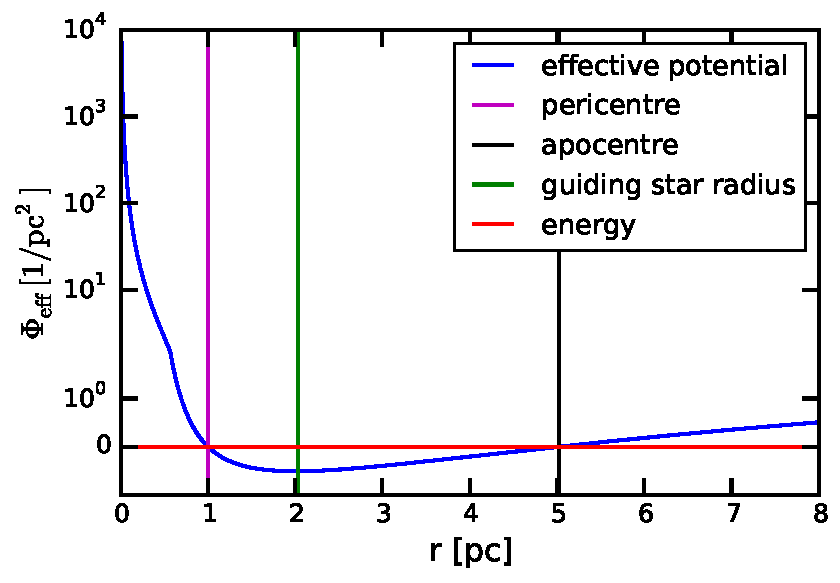
\includegraphics[width=\textwidth]{Plots/pot_eff_theory_part.pdf}
	\caption{Effective potential of a random star of SIM 1 (blue line). The total energy of the star (red line) is -1.88e-24 \(\mathrm{pc}^2/\mathrm{s}^2\). The intersections of energy and effective potential are the peri- and the apocentre of the star (magenta and black lines) and the minimum of the effective potential (green line) is the guiding star radius.}
	\label{pot_eff_theory_part}
	\end{subfigure}
\caption{Effective potentials.}
\label{fig:pot_eff_theory}
\end{figure}
\subsection{Integrals of motion}\label{int_of_motion_theory}
\subsection{Orbits \& orbit integration}\label{orbit_theory}
\color{red} how does the orbit in a spherical potential look\\include effective potential\\ \color{black}
In a dynamical system the mass distribution is described by the form of theoretically existent orbits (\(\vec{x}(t),\vec{v}(t))\). Position and velocity are linked with six coordinates and contain all information about the potential. With Newton's 2nd law we get the connection between potential \(\Phi(\vec{r})\)and acceleration \(\vec{a}\) which is \[\vec{F}(\vec{r})=-\nabla\Phi(\vec{r})=m\cdot\vec{a}.\] Since the system is spherically potential and force only depend on the distance from the centre r. The potential can be derived from the Poisson's equation \begin{equation}
\Delta\Phi(r)=4\pi G \rho(r)
\end{equation}
with the density \(\rho\) depending only on the distance as well. Due to the spherical symmetry the potential can be calculated by 
\begin{equation}
\Phi(r)=-\frac{G}{r}\int_0^r{\mathrm{d}M(r')}-G\int_r^{\infty}{\frac{\mathrm{d}M(r')}{r'}}=-4\pi G\left[\frac{1}{r}\int_0^r\mathrm{d}r'r'^2\rho(r')+\int_r^{\infty}\mathrm{d}r'r'\rho(r')\right]
\end{equation} (Binney \& Tremaine eq. 2.28). We calculate the density by binning the masses on logarithmic equally distributed shells \color{red} write density formula? \color{black} and solve the integrals of the Poisson's equation numerically by using the Gauss-Legendre quadrature \[\int_a^b f(x)dx = \frac{b-a}{2}\sum_{i=1}^n w_i f\left(\frac{b-a}{2}x_i+\frac{a+b}{2}\right)\] where the points \(x_i\) and the weights \(w_i\) are derived from the Legendre polynomials.\\ Since the orbit is described by position and velocity at each time step we use the numerical leapfrog method which is a second-order time reversible integrator. \(X_i\) and \(v_i\) are calculated by 
\begin{align*}
x_{i+1}=x_i+v_i\Delta t+\frac{a_i(x_i)}{2}\Delta t^2 \\
v_{i+1}=v_i+\frac{a(x_{i+1})+a(x_i)}{2}\Delta t.
\end{align*}

\color{red} gcs are collisional clusters but we assume them as collisionless \\ time evolution of actions \color{black}


\subsection{Actions}
Stars in spherical symmetric potential are fully described by their actions \begin{equation}
J_i=\frac{1}{2\pi}\oint_{\gamma_i}\vec{p}\cdot d\vec{q} \qquad\qquad i=r,\theta,\phi
\end{equation} which are used as coordinates in action space
These actions are integrals of motion. For most potentials actions can't be described analytically. The actions of a spherical system are derived from angular momentum, energy and potential. Only the potential is depending in r. Energy and angular momentum as well as resulting actions are constant over time and orbit. The azimuthal action J\(_\phi\) and the latitudinal action J\(_\theta\) can be evaluated simply. To calculate the radial action J\(_r\) we have to solve an integral numerically. Actions of a spherical potential are found to be \begin{align}
J_\phi=L_z, \\ J_\theta=L-|L_z|, \\ J_r=\frac{1}{\pi} \int_{r_{min}}^{r_{max}} \mathrm{d}r \sqrt{2E-2\Phi(r)-\frac{L^2}{r^2}}.
\end{align}\color{red} Should I write down the derivation of the actions (B\&T p.220) or just the results (B\&T p.221, 3.221,3.223,3.224)?\color{black} \\ The pericenter \(r_{min}\) and the apocenter \(r_{max}\) as well as the guiding star radius \(r_g\) can be found in the effective potential \begin{equation}
V_L(r)=V(r)+\frac{L^2}{2mr^2}.\  \color{red} \mathrm{m\ should\ be\ left\ out\ right?} \color{black}
\end{equation} \color{red} Bartelman Theo 1 Skript p59 formula 6.27. \\ \color{black} In the peri- and apocenter the effective potential equals the total energy since the stars do not have any kinetic energy there. That results in following function which is to solve: \[\left(\frac{1}{r}\right)^2+\frac{2\cdot (\Phi-E)}{L^2}=0.\] \\ The guiding star radius is the distance at which a star with given total angular momentum would have a circular orbit. This is at the minimum of the effective potential. To get \(r_g\) we have to solve \[r\sqrt{r\frac{\partial\Phi}{\partial r}}-|L|=0\] where \(\sqrt{r\frac{\partial\Phi}{\partial r}}=v_{circ}\) is the circular velocity. This distance is used to have a better comparison of the actions since in the snapshot the stars are at a random position on their orbit.

\color{red} plot v\_eff plot from barthelman skript? \color{black}
